\documentclass[tikz,border=6pt]{standalone}
\usepackage{times}
\usepackage{pgfplots}
\pgfplotsset{compat=1.18}
\begin{document}
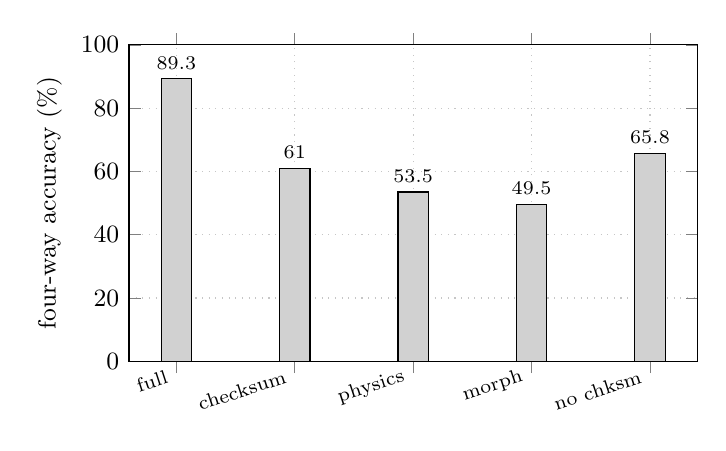
\begin{tikzpicture}
\begin{axis}[
  ybar,
  bar width=11pt,
  width=8.8cm,
  height=5.6cm,
  ylabel={four-way accuracy (\%)},
  ymin=0, ymax=100,
  symbolic x coords={full,checksum,physics,morph,no chksm},
  xtick=data,
  x tick label style={font=\scriptsize, rotate=18, anchor=east},
  nodes near coords,
  nodes near coords style={font=\scriptsize, /pgf/number format/fixed, /pgf/number format/precision=1},
  grid=major,
  major grid style={dotted, gray!45},
  tick label style={font=\small},
  label style={font=\small},
]
\addplot[fill=black!18, draw=black] coordinates {
  (full,89.3) (checksum,61.0) (physics,53.5) (morph,49.5) (no chksm,65.8)
};
\end{axis}
\end{tikzpicture}
\end{document}
